\chapter{Software Specification} 
\label{chap:requirements} 

\citet{cadle10} states that there is a standard hierarchical approach in
structuring requirements. Table \ref{table:requirementsCategories} outlines the
main four categories:

\begin{table}[H]   
  \begin{tabular}{|l|l|l|l|}
  \hline     
  {\bf General}        & {\bf Technical}  & {\bf Functional} & {\bf Non-Functional}    \\ 
  \hline
  Business constraints & Hardware         & Data entry       & Performance             \\      
  Business policies    & Software         & Data maintenance & Security                \\      
  Legal                & Interoperability & Procedure        & Legal and Access        \\      
  Branding             & Internet         & Retrieval        & Backup and Recovery     \\      
  Cultural             & ~                & ~                & Archiving and Retention \\      
  Language             & ~                & ~                & Maintainability         \\      
  ~                    & ~                & ~                & Business Continuity     \\      
  ~                    & ~                & ~                & Availability            \\      
  ~                    & ~                & ~                & Usability               \\      
  ~                    & ~                & ~                & Capacity                \\     
  \hline   
  \end{tabular}
  \label{table:requirementsCategories} 
\end{table}


Although these are some of the sections usually found in the structure of
requirements there are several books which state that each section depends on
the type of project being undertaken. 

\citet{robertson13} mentions that `a requirement is something the product must 
do to support its owners business, or a quality it must have to make it 
acceptable and attractive to the owner.' The aim of gathering the requirements 
has always been to ensure that all ambiguities are removed before a product is 
developed. 

As well as the process of requirements engineering there are standards available
for organizations to adhere to when compiling their documents. A more common
standard is the ISO 9001 for Quality Assurance. In the document it is described
that an organizations system is influenced by:

\begin{itemize}
  \item its organizational environment, changes in that environment, and the 
        risks associated with that environment
  \item its varying needs
  \item its particular objectives
  \item the products it provides
  \item the processes it employs
  \item its size and organizational structure
\end{itemize}
\hfill\citep{iso08}

As the project consists of four members whom are part of all development teams 
such standards do not need to be followed but an awareness of these standards is
beneficial. The advantage of a standard such as the ISO 9001 would be to the
project would be only if the project is integrated as a business outside the
scope of University studies.

The following sections have been derived from the book by \citet{robertson13}.
The book contains a very useful template called the Volere template which aims
to recognize as much information required when engineering requirements.


% Project Drivers % Purpose 
%\newpage
%\section{Purpose}

\subsection{Background of the Project}

The purpose of this project is to produce an app that will be compatible with the three main mobile operating systems, iOS, Android and Blackberry OS. The app is to be able to solve given clues from cryptic crosswords which are widely available on publications such as the Burgundian newspaper. There is no current form mobile application in the current market which solves cryptic clues. The produced product is to allow the end user to solve some if not all types of clues which have been discussed in section 2.1.3.

\subsection{Project Goals}

The main goals of the project are:

\begin{enumerate}
  \item Solve a given clue
  \item Produce a mobile interface which shows a stack trace of how the clue was deduced
\end{enumerate}



% Client, customer and stakeholder 
%\newpage
%\section{The Client, the Customer and Other Stakeholders}

\subsection{The Client}

 % Client
	\textbf{Dr Hugh \textsc{Osborne}}\\
	Senior Lecturer\\
	University Of Huddersfield\\
	h.r.osborne@hud.ac.uk

\subsection{The Customer}

The intended customer of the product are users of smartphone and tablets whom are looking to solve all those unsolvable Cryptic Crosswords. The applications will be deployed on the app market for the three listed mobile operating systems which means that the app will be available to anyone who has a compatible device with the required software. The physical deployment of the application is out of the project scope so a price for the deployment will not be discussed.

\subsection{Other Stakeholders}

For the purpose of the project the other stakeholders are as follows:

 % Supervisor
      \emph{Project Supervisor}\\
      \textbf{Dr. Gary \textsc{Allen}} \\
      Senior Lecturer \\
      University Of Huddersfield \\
      g.allen@hud.ac.uk 

  % Examiner
      \emph{Project Examiner:} \\ 
      \textbf{Sotirios \textsc{Batsakis}}\\
      University Of Huddersfield\\
      s.batsakis-STA@unimail.hud.ac.uk

  % Moderator
      \emph{Internal Moderator}\\
      \textbf{Collin \textsc{Venters}} \\
      Senior Lecturer \\
      University Of Huddersfield \\
      c.venters@hud.ac.uk



% Aims and Objectives
\newpage
%%%
%% Specification :: Aims & Objectives ::
%%%
\section{Aims \& Objectives}


%%%
%% Specification :: Aims & Objectives :: Aims
%%%
\subsection{Aims}

\begin{itemize}
  \item Produce a software application that accepts the input of cryptic 
        crossword clues from a user
  \item Produce a software application that will present a set of results to a
        user for the cryptic crossword clue which has been input
  \item Effectively adhere to a project plan as a team
  \item Effectively abide by the guidelines of a chosen software methodology
  \item Construct systematic and comprehensive documentation for the academic
 report
\end{itemize}


%%%
%% Specification :: Aims & Objectives :: Objectives
%%%
\subsection{Objectives}

\begin{itemize}
  \item To research cryptic crosswords themselves and the various types of 
        cryptic crossword clue
  \item To study relevant software architectures associated with the group 
        project
  \item To investigate the field of artificial intelligence, in particular 
        natural language processing and justify the need for it within the 
        project to solve cryptic crossword clues
  \item To research the various software methodologies which exist and select 
        the most appropriate for the project
  \item To understand and effectively follow a collection of requirements
  \item Evaluate the progress of the project at numerous instances throughout 
        the life cycle of the project
\end{itemize}

% Project Constraints % Mandated Constraints 
\newpage
\newpage
\section{Mandated Constraints}

The following section describes the constraints that effect the design of the
product. The product that is to be developed cannot be successful unless these
constraints have been accomplished.

%Solution Constraints
\subsection{Solution Constraints}

\noindent\llap{\textbf{[R1/1]}}The product shall be built for the following platforms:\\
\begin{enumerate}
		\item Blackberry
		\item iOS 
		\item Android
\end{enumerate}

\textbf{Rationale:}  The product it to be able to be used on the go.\\
\textbf{Volatility:} High


\noindent\llap{\textbf{[R2/1]}}The product shall require an Internet connection. \\

\textbf{Rationale:}  The product cannot work without an Internet connection.\\
\textbf{Volatility:} High

%Implementation Environment of the System
\subsection{Implementation Environment of the System}

\noindent\llap{\textbf{[R3/1]}}The product shall run on the following operating systems:\\

\begin{enumerate}
		\item Blackberry 10.2
		\item iOS 7
		\item Android 4.2 Jellybean
\end{enumerate}

\textbf{Rationale:}  The product is new therefore run on the latest software\\
\textbf{Volatility:} High

%Partner or Collaborative Applications
\subsection{Partner or Collaborative Applications}

\noindent\llap{\textbf{[R4/1]}}The product shall allow the user to login with their facebook account.

\textbf{Rationale:}  The product will allow a user to login in order to keep a search history, instead of creating a new authentication the user should be able to login using third part applications\\
\textbf{Volatility:} Low

%Off-the-Shelf Software
\subsection{Off-the-Shelf Software}

\noindent\llap{\textbf{[R5/1]}}The product shall make use of the Apache OpenNLP Library.

\textbf{Rationale:}  In order for the product to recognize the clues the best possible technique is to use Natural Language processing tools.\\
\textbf{Volatility:} Medium

%Schedule Constraints
\subsection{Schedule Constraints}

\noindent\llap{\textbf{[R6/1]}}The product shall be completed on or before the 18th April 2014.

\textbf{Rationale:}  The final deadline for all deliverables are 18/04/2014. \\
\textbf{Volatility:} High

%Budget Constraints
\subsection{Budget Constraints}

\noindent\llap{\textbf{[R7/1]}}The product shall be developed using all freely available tools and the only constraint of budget shall be the time the project resources put into to the product.

\textbf{Rationale:}  As the resources of the project are students, the product needs to be developed using the least amount of money as possible. The necessary steps should be taken to ensure that no costs are accumulated while developing the product \\
\textbf{Volatility:} Medium


% Relevant_Facts_And_Assumptions 
\section{Relevant Facts and Assumptions}

\subsection{Facts}

\noindent\llap{\textbf{[I1/1]}}Answers to Cryptic Crosswords are usually published the following day

\noindent\llap{\textbf{[I2/1]}}The same clues does not always have the same answers

\noindent\llap{\textbf{[I3/1]}}Existing applications don't offer real time solvers

\noindent\llap{\textbf{[I4/1]}}Electronic solvers not available

\subsection{Assumptions}

\begin{enumerate}
\item Equipment needed to test the application on different platforms will be
available.
\item A server to host the web service will be available.
\item The Guardian has given permission to use their cryptic crossword data to use for
our test data.
\item Four team members working on the project throughout the year at approximately
25\% of their academic study time
\item Project scope will remain the same throughout the project
\end{enumerate}


% Naming_Conventions And Terminology  
%\newpage
%\section{Naming Conventions and Terminology}

The following section contains a glossary with the meanings of all names, acronyms, and abbreviations used by the stakeholders.

\newpage
\subsection{Definitions of All Terms}

\begin{table}
    \begin{tabular}{|l|l|}
    \hline
    Term/Acronym  & Definition                                                \\ \hline
    The Guardian  &  A newspaper with a website featuring cryptic  crosswords \\ \hline
    Blackberry    & A mobile phone platform by Blackberry                     \\ \hline
    iOS           & A mobile phone platform by Apple                          \\ \hline
    Android       & A mobile phone platform by  Google                        \\ \hline
    NLP           & Natural Language Processing                               \\ \hline
    SRS           & Software Requirements Specification                       \\ \hline
    App           & Short for application                                     \\ \hline
    ~             & ~                                                         \\ \hline
    ~             & ~                                                         \\ \hline
    ~             & ~                                                         \\ \hline
    ~             & ~                                                         \\ \hline
    ~             & ~                                                         \\ \hline
    ~             & ~                                                         \\ \hline
    ~             & ~                                                         \\ \hline
    \end{tabular}
\end{table}



% Functional Requirements

% Scope
\newpage
%%%
%% Specification :: Scope
%%%
\section{Scope}

%%%
%% Specification :: Scope :: Organisation Structure
%%%
\subsection{Organisation Structure}

The project team is based largely upon democratic discussions and decisions,
however to ensure that team deadlocks do not occur a project leader has been
chosen. Figure ~\ref{fig:org_hierachy} reflects the hierarchy of the team.

\begin{figure}[H]
  \centering
  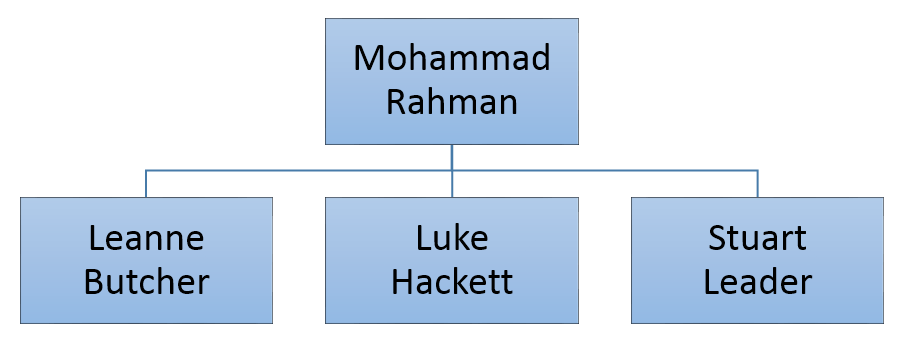
\includegraphics[width=0.9\textwidth]{organisation_structure.png}
  \caption{Hierarchical Structure of the team}
  \label{fig:org_hierachy}
\end{figure}


%%%
%% Specification :: Scope :: Organisation Structure :: Methodology
%%%
\subsection{Methodology}

It has been decided that the team will follow an Agile software development
model. This will allow the team to split the larger task down into smaller, more
manageable `chunks', that allows for a good quality analysis, evaluation,
development and planning (on to the next `chunk'). An iterative approach is best
suited for this project due to the nature of changes and updates the product
will require in future builds.

This method of development also allows for a more feature-driven approach to the
project. Ultimately this allows for more important features and aspects of the
project to be completed first.


%%%
%% Specification :: Scope :: Meetings
%%%
\subsection{Meetings}

A weekly meeting will take place between all project members to discuss all
aspects of the project. This includes (but is not limited to) project issues,
software development issues, research findings, possible improvements and code
reviews.


%%%
%% Specification :: Scope :: Product
%%%
\subsection{Product}

Within the cryptic crossword area, there is a need for a cryptic crossword clue
solver in the form of a software application.  This has been justified
previously within the document through research and investigating existing
applications within the field. The main purposes of the software deliverable are
to allow the input of a cryptic crossword clue by a user and output a potential 
results or number of results.

Once the project has been completed by the team, the following deliverables will
have been accomplished:

\begin{itemize}
  \item A software application which accepts input from the user and outputs 
        appropriate solutions. 
  \item Two written reports that:
    \begin{itemize}
      \item document the entire software development process from a group 
            perspective
      \item analyse and evaluate the project as a whole
    \end{itemize}
\end{itemize}

Furthermore the subsequent internal components will be implemented to aid with 
the goals of the project:

\begin{itemize}
  \item A storage area to collect and store the cryptic crossword clues and 
        their details used for test data as well as, clues successfully solved 
        by the application which a user has input.
  \item A service which will allows connections from web browsers and 
        potentially mobile phones to ensure the running of the software 
        application.
\end{itemize}

There are specific criteria which have been identified as important features
which must be completed to deem the project as adequately finished:

\begin{itemize}
  \item A document outlining the full software development life cycle of the 
        project
  \item A software application which can be accessed via either:
    \begin{itemize}
      \item A web browser \textbf{and/or}
      \item A portable device (e.g. smartphone or tablet)
    \end{itemize}
  \item A service which can be connected to by either a mobile phone or a web 
        browser which will sufficiently solve a cryptic crossword clue and 
        output a result or number of results 
  \item A storage area accessible by the service which stores the cryptic 
        crossword clues and their associated details
\end{itemize}

Furthermore, there are specific criteria which have been deemed as out of the 
scope of the project:

\begin{itemize}
  \item The user will not be able to access the storage area to browse through 
        data
  \item The software application will not be implemented to have the ability to
        generate cryptic crosswords from the data stored
\end{itemize}

The restrictions listed below are the justifications for the project scope:

\begin{itemize}
  \item The time scale of the project
  \item External priorities from the academic year such as other module 
        assignments and examinations
  \item Limited resources for testing the software application on restrict the
        platforms which the software application will be fully compatible with
\end{itemize}


% Business Data Model & Data Dictionary 
%\newpage 
%\section{Business Data Model \& Data Dictionary}

% The Scope of the Product 
%\newpage
%\section{The Scope of the Product}

\subsection{Use case Diagrams}

% Functional Requirements 
\newpage
\section{Functional Requirements}


\subsection{Data entry}

\subsection{Data maintenance}

\subsection{Procedure}

\subsection{Retrieval}



% Non-functional Requirements 
\newpage
\section{Non-Functional Requirements}

\subsection{Performance}

The performance of the system should be good, however it must be noted that the
system is intended to run as a web service upon a server. The quality of the 
connection between the end user and the web service will be out of the scope of
this project.


\subsection{Legal and Access}

Within the project a number of data sources will be used. Firstly an English
dictionary will need to be accessed in order to allow the system to deduce if a 
given arrangement of characters formulates an English word.

In order to achieve this, an offline dictionary and an online dictionary will
need to be used. The offline dictionary is a short dictionary and is provided as
part of the GNU/Linux operating system under the GNU Licence Agreement. The 
online dictionary will be used to `fill in' any gaps in the short dictionary.
*** Offline Dictionary Licence to be added here ***

A number of cryptic crossword clues and solutions have been obtained from the
Guardian's website. The data will be used as a training set of data, when
testing the final software. The Guardian has given us permission to use their
data as long as the project remains within an academic environment, and that no
profit is made from the project.


\subsection{Backup and Recovery}

The project will make use of the git revision control system over a secure shell 
connection. The service provider is github, who offer a distributed setup to 
ensure that data is always available. Using a secure revision control system 
will ensure that:

\begin{enumerate}
  \item A copy of the project is stored upon a remote, secure server;
  \item Changes are able to be tracked;
  \item Issues and comments are able to be raised in a secure environment.
\end{enumerate}

The above measures will in effect be able to reduce against the loss, damage or 
theft of all project information.


\subsection{Archiving and Retention}

The University will retain a copy of the project (software product and the final
report) for assessment and evaluation purposes. 


\subsection{Maintainability}

The project -- including the software product -- will be maintained up until the
project hand in deadline: 18th April 2014.


\subsection{Availability}

The software will not contain any request or time limitations for users, and 
thus should be available at all times. However it must be stated that the server
availability that will be hosting the web service is out of the scope of the 
project.


\subsection{Capacity}

The end product should be able to handle a number of requests from different 
users at the same time. As the project is only intended as an academic project, 
large scale user support will be out of the scope of this project.


\section{Usability and Humanity Requirements}

%Look and Feel Requirements 
%\newpage
%\section{Look and Feel Requirements}

%Usability and Humanity Requirements 
%\newpage 
%\section{Usability and Humanity Requirements}

%Performance Requirements 
%\newpage
%\section{Performance Requirements}

% Operational and Environmental Requirements 
%\newpage 
%\section{Operational and Environmental Requirements}

%Maintainability and Support Requirements 
%\newpage 
%\section{Maintainability and Support Requirements}

%Security Requirements 
%\newpage
%\section{Security Requirements}

%Cultural Requirements 
%\newpage
%\section{Cultural Requirements}

%Legal Requirements 
%\newpage
%\section{Legal Requirements}

%Project Issues 
%Open Issues 
%\newpage
%\section{Open Issues} 

%Off-the-Shelf Solutions
%\newpage 
%\section{Off-the-Shelf Solutions}

%New Problems 
%\newpage 
%\section{New Problems}

%Tasks 
%\newpage 
%\section{Tasks}

%Migration to the New Product 
%\newpage
%\section{Migration to the New Product}

%Risks 
\newpage 
\section{Risk Assessment}

% Introduction.
An investigation into the potential risks that may present themselves during the course of this project is of paramount importance if their impact is going to be minimised, should they become a reality.

% Included here a risk impact table
\subsection{Risk Identification}

% PI Scores and risk classification graph
\subsection{Risk Classification}

\subsection{Risk Prevention}

\subsection{Risk Mitigation}

%Costs 
%\newpage 
%\section{Costs}

%User Documentation and Training 
%\newpage
%\section{User Documentation and Training}

%Waiting Room 
%\newpage 
%\section{Waiting Room}

%Ideas for Solutions 
%\newpage
%\section{Ideas for Solutions}


